\documentclass{beamer}

\author{李昊泽}
\title{基础数据结构选讲}
\date{2025年10月7日}
\usepackage{hit-style}
\usepackage[minted,fira,siyuan]{hit-extra}

\begin{document}

\begin{frame}
    \titlepage
\end{frame}

\begin{frame}
    \tableofcontents[sectionstyle=show,subsectionstyle=show/shaded/hide,subsubsectionstyle=show/shaded/hide]
\end{frame}

\section{线性表}
\subsection{栈}
\subsubsection{引入}
\begin{frame}{洗碗问题}
    \begin{minipage}[c]{0.5\linewidth}
        小泽是餐厅里的洗碗工。

        每天都有堆积如山的盘子需要他洗。他每次从这叠盘子里面取出最顶上的那一个,然后把它洗干净,放到别的地方。

        恰饭的人源源不断,所以需要洗的盘子也源源不断地送过来。每次来了新的盘子,都会被放在那叠盘子的最顶上。\\

        \textbf{如何用一个数组模拟这叠盘子?}
    \end{minipage}
    \begin{minipage}{0.4\linewidth}
        \begin{figure}
            \begin{center}
                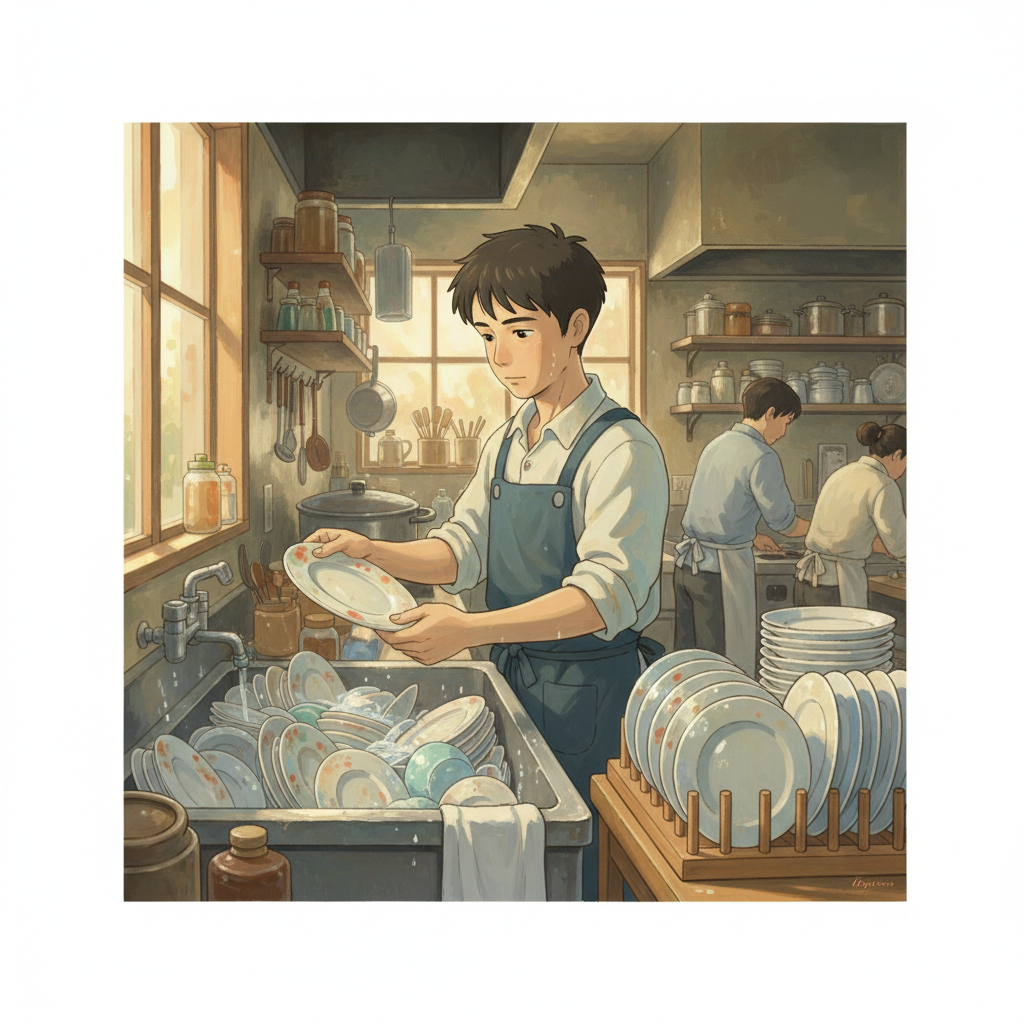
\includegraphics[width=\linewidth]{./pic/Gemini_Generated_Image_4uekal4uekal4uek.png}
                \caption{小泽洗碗图}
            \end{center}
        \end{figure}
    \end{minipage}
\end{frame}

\begin{frame}{洗碗问题}
    \begin{center}
    \begin{tabular}{cc}
        \toprule
        事件 & 状态 \\
        \hline
        放入 $1$ & $1$ \\
        放入 $2$ & $1, \ 2$ \\
        放入 $3$ & $1, \ 2, \ 3$ \\
        取出顶端($3$)& $1, \ 2$ \\
        取出顶端($2$) & $1$ \\
        放入 $4$ & $1, \ 4$ \\
        放入 $5$ & $1, \ 4, \ 5$ \\
        取出顶端($5$) & $1, \ 4$ \\
        取出顶端($4$) & $1$ \\
        取出顶端($1$) & 空 \\
        \bottomrule
    \end{tabular}
    \end{center}
\end{frame}

\subsubsection{栈的性质}
\begin{frame}{栈的性质}
    在前面的引入中,我们发现:盘子都是从顶端进,从顶端出。如果 a 比 b 早进入,那么 a 一定比 b 后退出\\

    这个性质即为“后进先出”,它是 \textcolor{red}{栈} 的本质。 \\

    \textbf{栈} (stack):LIFO(Last In, First out)表 \\
\end{frame}

\subsubsection{栈的实现}
\begin{frame}[fragile]{实现栈}
    \begin{minipage}[t]{0.4\linewidth}
        C-style 模拟
        \begin{minted}{cpp}
            int stk[N], top = 0;
            // 向栈顶插入一个数
            stk[++top] = x;
            // 从栈顶弹出一个数
            top--;
            // 获取栈顶的值
            stk[top];
            // 判断栈是否为空
            if (top > 0) { }
        \end{minted}
    \end{minipage}
    \hspace{1cm}
    \begin{minipage}[t]{0.4\linewidth}
        STL 模拟
        \begin{minted}{cpp}
            std::vector<int> stk;
            // 向栈顶插入一个数
            stk.push_back(x);
            // 从栈顶弹出一个数
            stk.pop_back();
            // 获取栈顶的值
            stk.back();
            // 判断栈是否为空
            if (!stk.empty()) { }
        \end{minted}
    \end{minipage}
\end{frame}

\begin{frame}
    事实上,在 STL 中存在标准的 \mintinline{cpp}{std::stack} 实现,其内部使用 \mintinline{cpp}{std::deque} 实现,所以有较大的常数,并且其不支持随机访问,所以我们使用 \mintinline{cpp}{std::vector} 来模拟栈。
\end{frame}

\subsubsection{例题}
\begin{frame}{例题一(Luogu B3614)}
    请你实现一个栈(stack),支持以下操作:
    \begin{enumerate}
        \item \mintinline{cpp}{push(x)}: 向栈中加入一个数 $x$。
        \item \mintinline{cpp}{pop()}: 将栈顶输出。如果此时栈为空则不进行弹出操作,输出 \mintinline{cpp}{Empty}。
        \item \mintinline{cpp}{query()}: 输出栈顶元素,如果此时栈为空则输出 \mintinline{cpp}{Anguei!}。
        \item \mintinline{cpp}{size()}: 输出此时栈内元素个数。
    \end{enumerate}
\end{frame}

\begin{frame}[fragile]{代码}
    此处使用 \mintinline{cpp}{std::vector} 进行栈的模拟。

    以下仅展示核心逻辑部分的代码。

    \begin{minted}[fontsize=\footnotesize]{cpp}
if (op == "push") {
    u64 x;
    std::cin >> x;
    stk.push_back(x);
} else if (op == "pop") {
    if (stk.empty()) {
        std::cout << "Empty\n";
    } else {
        stk.pop_back();
    }
} else if (op == "query") {
    if (stk.empty()) {
        std::cout << "Anguei!\n";
    } else {
        std::cout << stk.back() << "\n";
    }
} else {
    std::cout << stk.size() << "\n";
}
    \end{minted}
\end{frame}

\begin{frame}{例题二 \ 括号匹配问题(UVA 673)}
    给定一串由 () 和 [] 组成的字符串,我们规定以下的字符串是合法的字符串:
    \begin{enumerate}
        \item 空串是合法的
        \item 如果 A、B 都是合法的,那么 AB 是合法的
        \item 如果 A 是合法的,那么 (A) 和 [A] 都是合法的
    \end{enumerate}
    请写出一个程序,判断每一个给定的字符串是否合法。
\end{frame}

\begin{frame}{分析}
    我们可以先手玩一下以下的字符串是否合法:

    \begin{itemize}
        \item \mintinline{text}{[(())]}
        \item \mintinline{text}{()[]()}
        \item \mintinline{text}{[([])[]]()}
        \item \mintinline{text}{(()}
        \item \mintinline{text}{([)(])}
    \end{itemize}

    将一个字符串从左往右写,一旦遇到匹配上的括号,就把这对括号擦掉。
\end{frame}

\begin{frame}
    我们可以使用一个栈来维护上面的操作。

    当新加入一个括号时:

    \begin{enumerate}
        \item 如果是左括号,则把这个括号入栈
        \item 如果是右括号,看栈顶是否能和这个右括号匹配,如果可以的话弹出栈顶,否则这个字符串不合法
    \end{enumerate}
\end{frame}

\begin{frame}[fragile]{代码}
    完整代码见 \href{https://vjudge.net/solution/64150195/NWv7brPjI5uhjS91FLfu}{vjudge 提交记录}

    \begin{minted}[fontsize=\footnotesize]{cpp}
for (int i = 0; i < s.length(); i++) {
    if (s[i] == '(' or s[i] == '[') {
        stk.push_back(s[i]);
    } else {
        if (not stk.empty() and s[i] == ')' and stk.back() == '(') {
            stk.pop_back();
        } else if (not stk.empty() and s[i] == ']' and stk.back() == '[') {
            stk.pop_back();
        } else {
            std::cout << "No\n";
            return;
        }
    }
}
if (not stk.empty()) {
    std::cout << "No\n";
} else {
    std::cout << "Yes\n";
}
    \end{minted}
\end{frame}

\begin{frame}{例题三 \ 后缀表达式}
所谓后缀表达式是指这样的一个表达式:式中不再引用括号,运算符号放在两个运算对象之后,所有计算按运算符号出现的顺序,严格地由左而右新进行(不用考虑运算符的优先级)。

本题中运算符仅包含 $+ - * /$。保证对于 $/$ 运算除数不为 $0$。特别地,其中 $/$ 运算的结果需要向 $0$ 取整(即与 C++ $/$ 运算的规则一致)。

如:$3*(5-2)+7$ 对应的后缀表达式为:$3.5.2.-*7.+@$。在该式中,$@$ 为表达式的结束符号。$.$ 为操作数的结束符号。
\end{frame}

\begin{frame}{分析}
    后缀表达式不需要使用括号,其运算方案是唯一的。对于计算机来说,最容易理解后缀表达式。\\

    \fbox{
        \parbox{\textwidth}{
            \centering
            \textbf{后缀表达式求值}

            \begin{enumerate}
                \item 建立一个用于存数的栈,逐一扫描该后缀表达式中的元素。
                \begin{enumerate}
                    \item 如果遇到一个数,则把该数入栈
                    \item 如果遇到运算符,就取出栈顶的两个数进行计算,把结果入栈
                \end{enumerate}
                \item 扫描完成后,栈中恰好剩下一个数,就是该后缀表达式的值
            \end{enumerate}
        }
    }
\end{frame}

\begin{frame}[fragile]{代码}
    由于该题的逆天输入格式,这里使用 Java 代码演示主要逻辑:

    \begin{minted}[fontsize=\footnotesize]{java}
Pattern p = Pattern.compile("(\\d+|[+\\-*\\/])");
Matcher m = p.matcher(s);

Stack<Integer> stk = new Stack<>();
while (m.find()) {
    String x = m.group(1);
    if (x.matches("\\d+")) {
        stk.push(Integer.parseInt(x));
    } else {
        int b = stk.peek();
        stk.pop();
        int a = stk.peek();
        stk.pop();
        stk.push(
            switch (x) {
                case "+" -> a + b;
                case "-" -> a - b;
                case "*" -> a * b;
                case "/" -> a / b;
                default -> 0;
            }
        );
    }
}
System.out.println(stk.peek());
    \end{minted}
\end{frame}

\subsubsection{课后作业}
\begin{frame}{课后作业}
    \begin{itemize}
        \item 最小栈 \href{https://leetcode.cn/problems/min-stack/}{LeetCode 155} (栈的灵活应用)
        \item Editor \href{https://acm.hdu.edu.cn/showproblem.php?pid=4699}{HDU 4699}(对顶栈)
        \item \string[NOIP 2013 普及组\string] 表达式求值 \href{https://www.luogu.com.cn/problem/P1981}{Luogu P1981} (中缀表达式求值)
        \item \string[河南省第十五届ICPC大学生程序设计竞赛\string] 表达式求导 (中缀表达式递归求值)
        \item \string[NOIP 2003 普及组\string] 栈 \href{https://www.luogu.com.cn/problem/P1044}{Luogu P1044} (栈的数学性质)
    \end{itemize}
\end{frame}

\begin{frame}
    \begin{center}
        {\Huge\calligra Thanks!}
    \end{center}
\end{frame}

\end{document}